\let\negmedspace\undefined
\let\negthickspace\undefined
\documentclass[journal,12pt,twocolumn]{IEEEtran}
\usepackage{cite}
\usepackage{amsmath,amssymb,amsfonts,amsthm}
\usepackage{algorithmic}
\usepackage{graphicx}
\usepackage{textcomp}
\usepackage{xcolor}
\usepackage{txfonts}
\usepackage{listings}
\usepackage{enumitem}
\usepackage{mathtools}
\usepackage{gensymb}
\usepackage{comment}
\usepackage[breaklinks=true]{hyperref}
\usepackage{tkz-euclide} 
\usepackage{listings}
\usepackage{gvv}                                        
\def\inputGnumericTable{}                                 
\usepackage[latin1]{inputenc}                                
\usepackage{color}                                            
\usepackage{array}                                            
\usepackage{longtable}                                       
\usepackage{calc}                                             
\usepackage{multirow}                                         
\usepackage{hhline}                                           
\usepackage{ifthen}                                           
\usepackage{lscape}
\usepackage{caption}

\newtheorem{theorem}{Theorem}[section]
\newtheorem{problem}{Problem}
\newtheorem{proposition}{Proposition}[section]
\newtheorem{lemma}{Lemma}[section]
\newtheorem{corollary}[theorem]{Corollary}
\newtheorem{example}{Example}[section]
\newtheorem{definition}[problem]{Definition}
\newcommand{\BEQA}{\begin{eqnarray}}
\newcommand{\EEQA}{\end{eqnarray}}
\newcommand{\system}[1]{\stackrel{#1}{\rightarrow}}
\newcommand{\define}{\stackrel{\triangle}{=}}
\theoremstyle{remark}
\newtheorem{rem}{Remark}
\begin{document}

\bibliographystyle{IEEEtran}
\vspace{3cm}

\title{Gate 2023-IN-21}
\author{EE22BTECH11008 - Annapureddy Siva Meenakshi$^{*}$% <-this % stops a space
}
\maketitle
\bigskip

\renewcommand{\thefigure}{\theenumi}
\renewcommand{\thetable}{\theenumi}
Q:A system has transfer function
 \[\frac{Y(s)}{X(s)}=\frac {s-\pi}{s+\pi}\]
 let $u(t)$ be the unit step function.The input $x(t)$ that results in a steady-state output $y(t)=sin(\pi t)$ is \underline{\quad}.
\solution
\begin{table}[!ht]
    \centering
        \input{./tables/table.tex}
    \caption{input parameters}
    \label{tab:in_21_t1}
\end{table}
 \begin{equation}
     H(s)=\frac{s-\pi}{s+\pi}
 \end{equation} 
 let 
 \begin{equation}
     H_i(s)=\frac{s+\pi}{s-\pi}
 \end{equation} 
 This is the Transfer function of inverse system having $y(t)$ as input and $x(t)$ as output.\\
 Converting transfer function to frequency response, we get
 \begin{equation}
     H_i(j\omega)=\frac{j\omega+\pi}{j\omega-\pi}
 \end{equation}
 Here , $\omega=\pi$
 \begin{align}
    H_i(j\pi)&=\frac{j+1}{j-1}=-j\\
     |H(j\pi)|&=1\\
    \angle H(j\pi)&=-90^\circ\\
    y(t)&=\sin(\pi t)\label{eq:in.21.6} 
\end{align}
\begin{align}
  |X|\sin(\omega t+\phi)&\system{H(j\omega)}|X||H(j\omega)|\sin(\omega t +\phi +\angle H(j\omega))\label{eq:in.21.7}\\
  \sin(\pi t)&\system{H(j\omega)}|H(j\omega)|\sin\left(\pi t  +\angle H(j\omega)\right)\label{eq:in.21.8}
\end{align}
Therefore by ~\eqref{eq:in.21.6} and ~\eqref{eq:in.21.8} , we get
\begin{equation}
    x(t)=\sin\left(\pi t -\frac{\pi}{2}\right)
\end{equation}

\begin{figure}[htb]
  \centering
  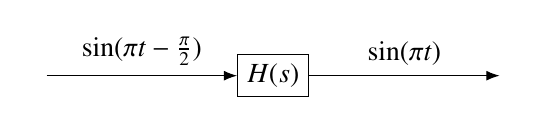
\begin{tikzpicture}[auto, node distance=4cm,>={Latex}]
  % Define blocks
  \node (input) at (0,0) {};
  \node [draw, rectangle] (H) at (3,0) {$H(s)$};
  \node (output) at (6,0) {};

  % Connect blocks with right arrows
  \draw [->] (input) -- node[midway, above] {$\sin(\pi t - \frac{\pi}{2})$} (H);
  \draw [->] (H) -- node[midway, above] {$\sin(\pi t)$} (output);
\end{tikzpicture}

  \captionsetup{justification=centering, singlelinecheck=off}
  \caption{Block diagram of the System}
  \label{fig:tikz_circuit}
\end{figure}

\begin{figure}[h]
  \centering
  \includegraphics[width=\columnwidth]{./figs/fig1.png} 
  \captionsetup{justification=centering}
  \caption{Plot of $x(t)$ and $y(t)$ taken from Python}
  \label{fig:your_label}
\end{figure}

 \end{document}
